\documentclass[11pt,xcolor=x11names,compress, notes=show]{beamer}% pour l'impression, tout n'apparait qu'une fois \documentclass[handout,12pt]{beamer}
\usepackage[utf8x]{inputenc}
\usepackage{ucs}
\usepackage[UKenglish]{babel}
\usepackage{todonotes}
\usepackage{tikz}
\usepackage{color}
\usepackage{subfigure}
\usetikzlibrary{calc}

\usepackage{bm}
\usepackage{pifont} %pour les symbole sympa \ding{nb}
\usepackage[export]{adjustbox}

\setbeamertemplate{navigation symbols}{} 


%\usepackage{palatino}

%pour le theme
%\usetheme{CambridgeUS}

%\usetheme{Goettingen}
\useinnertheme{default}
\useoutertheme[subsection=false]{miniframes}
\setbeamertemplate{blocks}[rounded][shadow=true]
\setbeamercolor{block title}{fg=DeepSkyBlue4,bg=DeepSkyBlue4!10}
\setbeamercolor{block title alerted}{bg=DeepSkyBlue4!0} 
\setbeamercolor{block title example}{bg=DeepSkyBlue4!20}
\setbeamercolor*{lower separation line head}{bg=DeepSkyBlue4} 

\setbeamerfont{title like}{shape=\scshape}
\setbeamercolor{frametitle}{fg=DeepSkyBlue4}
\setbeamercolor{title}{fg=DeepSkyBlue4}
\setbeamercolor{itemize item}{fg=black}
\setbeamercolor{itemize subitem}{fg=black}
\setbeamercolor{toc}{fg=DeepSkyBlue4}

%couleur table des matières
\usepackage{hyperref}
\hypersetup{colorlinks=true, linkcolor=DeepSkyBlue4}

%Mettre la section courante en titre de diapo (pour champ de titre non-vide)
%\addtobeamertemplate{frametitle}{\frametitle{\insertsubsectionhead}}{}

\addtobeamertemplate{footline}{\hspace{11cm} \insertframenumber/\inserttotalframenumber}

\author{Alice \textsc{Dinsenmeyer} \\~\\ supervised by \\ Romain \textsc{Brossier} \& Ludovic \textsc{Moreau}}

\title{FWI for Ultrasonic Imaging}
\subtitle{Flaw detection in steel weld}
\date{\small June 9, 2016}

\setbeamertemplate{caption}{\raggedright\insertcaption\par}

\begin{document}


\begin{frame}
	\titlepage 
\end{frame}


\section*{NDT for Welds}
\begin{frame}{\insertsectionhead}
\vspace{0.3cm}
	\begin{minipage}[c]{0.49\textwidth}
		\centering
		\begin{figure}
			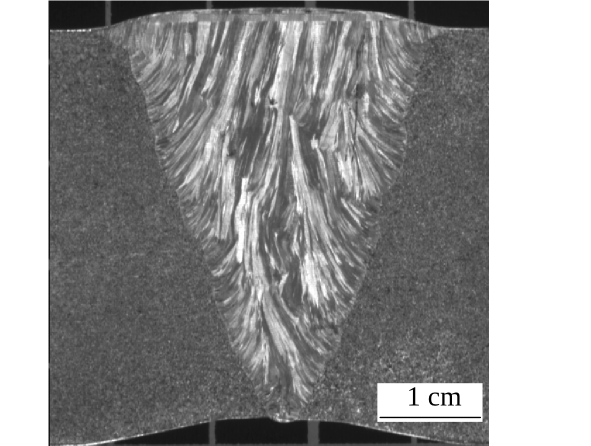
\includegraphics[height=2.7cm,right]{./img/soudure1.png}
			%\caption{\tiny (TV plane)}
		\end{figure}
	\end{minipage}
	%\hspace{0.3cm}
	\begin{minipage}[c]{0.49\textwidth}
		\centering
		\begin{figure}
			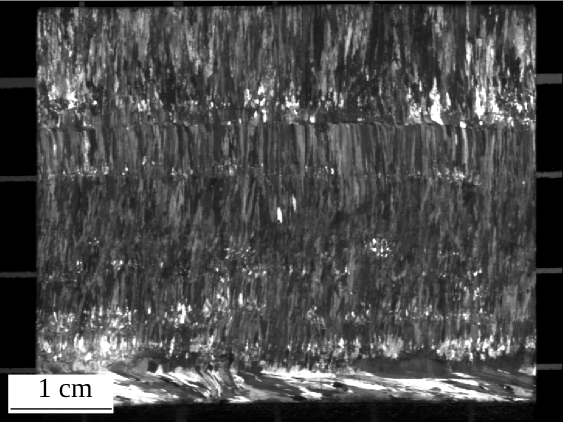
\includegraphics[height=2.7cm,left]{./img/soudure2.png}\\
			%\caption{\tiny (SV plane)}
		\end{figure}
	\end{minipage}
	\raggedleft{ \tiny Pictures from Chassignole 2000, PhD thesis}
	
	\begin{columns}[c]
			\column{.5\textwidth}<1->
			%\begin{block}{}
				\begin{itemize}
					\item[$\bullet$] delay and sum methods
					\item[$\bullet$] SVD decomposition of covariance matrix 
				\end{itemize}
			%\end{block}
			\column{.05\textwidth}<2->
			\ding{222}
			\column{.5\textwidth}<2->
			%\begin{block}{}
				\begin{itemize}
					\item[\ding{55}] need to know $c$ in advance
					\item[\ding{55}] strong artefacts
				\end{itemize}
			%\end{block}
			
	\end{columns}
	\vspace{0.5cm}
	\begin{columns}[c]
		\column{.5\textwidth}<3->
			\begin{itemize}
				\item[$\bullet$] solving NL optimization problem
			\end{itemize}
		\column{.05\textwidth}<3->
			\ding{222}
		\column{.5\textwidth}<3->
			\begin{itemize}
				\item[\ding{51}] elastic parameters reconstruction
			\end{itemize}			
	\end{columns}
	
	\vspace{0.5cm}
	\begin{itemize}
		\item[~]
		\begin{itemize}
			\item contour reconstruction : \emph{Dominguez et al.}, \emph{Rodriguez et al.}
			\item cartography : FWI
		\end{itemize}
	\end{itemize}


\end{frame} 

\section{What is specific to weld imaging ?}
\begin{frame}{\insertsectionhead}
	\begin{itemize}
		\item <1-> 2 free surfaces : more information $\leftrightarrow$ more non-linearities
		\item <2-> surface acquisition only 
		\item <3-> anisotropy $\rightarrow$ multi-parameter inversion ($C_{ij}\times$6)
	\end{itemize}
	\vfill
	\begin{figure}[!h]
		\centering
		\includegraphics<1-1>[scale=1]{img/soud1.pdf}
		\includegraphics<2-2>[scale=1]{img/soud2.pdf}
		\includegraphics<3-3>[scale=1]{img/soud3.pdf}
	\end{figure}

\end{frame}

\section{To do}
\begin{frame}{\insertsectionhead}
	\begin{itemize}
		\item <1-> acoustic approximation (mono/multiparameter)
		\begin{itemize}
			\item isotropic weld ($v_{p}$, $\rho$)
			\item VTI weld	~~~~~~($v_{p}$, $\rho$, $\epsilon$, $\delta$)
			\item TTI weld	~~~~~~($v_{p}$, $\rho$, $\epsilon$, $\delta$, $\theta$)
		\end{itemize}
		\item <2-> elastic inversion (mono/multiparameter : $C_{ij}\times$6)
		\begin{itemize}
			\item isotropic weld
			\item anisotropic weld
			\item true data
		\end{itemize}		
	\end{itemize}
\end{frame}

\section{Ongoing work}
\begin{frame}{\insertsectionhead}
	\begin{itemize}
		\item <1-> 2D acoustic approximation (mono/multiparameter)
		\begin{itemize}
			\item isotropic weld (\fcolorbox{DeepSkyBlue4!40}{DeepSkyBlue4!10}{$v_{p}$}, $\rho$)
			\item VTI weld	~~~~~~($v_{p}$, $\rho$, \fcolorbox{DeepSkyBlue4!40}{DeepSkyBlue4!10}{$\epsilon$}, $\delta$)
			\item TTI weld	~~~~~~($v_{p}$, $\rho$, $\epsilon$, $\delta$, $\theta$)
		\end{itemize}
		\item <2-> elastic inversion (mono/multiparameter : $C_{ij}\times$6)
		\begin{itemize}
			\item isotropic weld
			\item anisotropic weld
			\item true data
		\end{itemize}		
	\end{itemize}
\end{frame}

\end{document}